\chapter{Introduction}

\section{Host Organism}
\subsection{SteelSeries}
\subsubsection{Company history and Background}
Steel\textbf{Series}, a Danish manufacturer of gaming peripherals, was founded in 2001 by Jacob Wolff-Petersen. The company originally launched under the name Soft Trading, and made its mark with innovative gaming mousepads in the early 2000s. In 2007, Soft Trading rebranded to SteelSeries, reflecting its broadened focus beyond mousepads and into a full range of PC gaming accessories. Key milestones in SteelSeries' evolution include the 2008 acquisition of Ideazon, which brought the Zboard and World of Warcraft gaming keyboard into its portfolio and furthered its presence in the North American market.
The company grew rapidly in the 2010s, fueled by its involvement in the esports scene and partnerships with professional gamers. SteelSeries has since expanded its product line to include high-performance gaming mice, keyboards, headsets, and mousepads, becoming a leading brand in the gaming industry.

\subsubsection{Key Products and Technologies}
SteelSeries, renowned for its gaming peripherals and accessories, spanning several product categories. Its product portfolio includes:
\begin{itemize}
    \item \textbf{Gaming Mice:} High-precision mice with customizable buttons and sensors.
    \begin{figure}[h!]
    \centering
    \begin{subfigure}[b]{0.25\textwidth}
        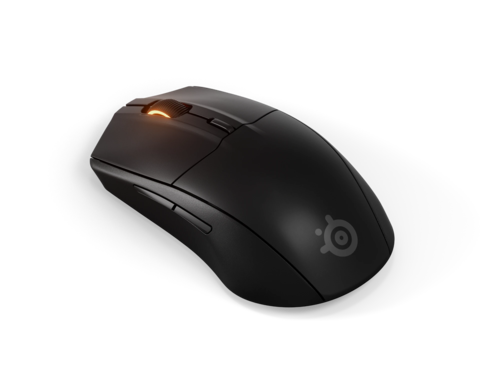
\includegraphics[width=\textwidth]{ressources/mouse_1.png}
        \caption{Rival 3 Wireless Gen 2}
    \end{subfigure}
    \hfill
    \begin{subfigure}[b]{0.25\textwidth}
        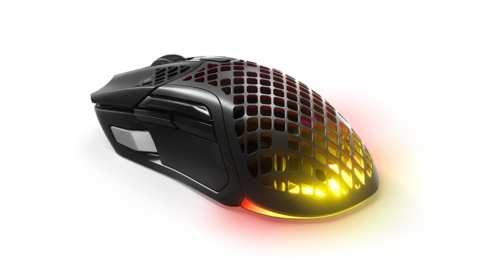
\includegraphics[width=\textwidth]{ressources/mouse_2.png}
        \caption{Aerox 5}
    \end{subfigure}
    \hfill
    \begin{subfigure}[b]{0.25\textwidth}
        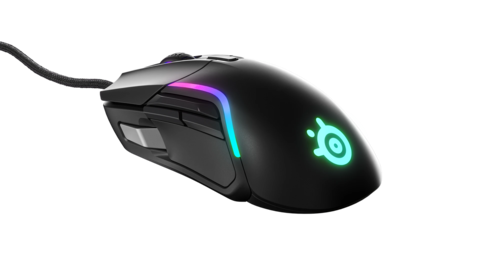
\includegraphics[width=\textwidth]{ressources/mouse_3.png}
        \caption{Rival 5}
    \end{subfigure}
    \caption{SteelSeries Gaming Mice}
    \end{figure}
    \item \textbf{Keyboards:} Mechanical and membrane keyboards designed for gaming performance.
    \begin{figure}[h!]
    \centering
    \begin{subfigure}[b]{0.25\textwidth}
        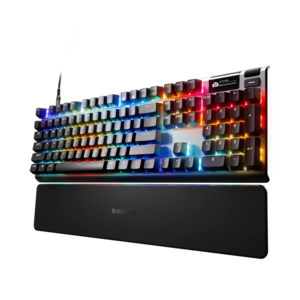
\includegraphics[width=\textwidth]{ressources/kb_1.png}
        \caption{Apex Pro Gen 3}
    \end{subfigure}
    \hfill
    \begin{subfigure}[b]{0.25\textwidth}
        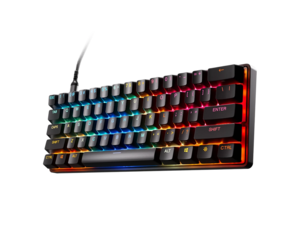
\includegraphics[width=\textwidth]{ressources/kb_2.png}
        \caption{Apex Pro Mini Gen 3}
    \end{subfigure}
    \hfill
    \begin{subfigure}[b]{0.25\textwidth}
        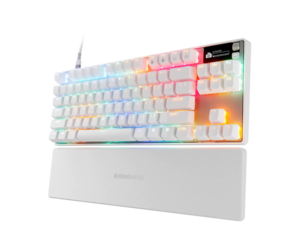
\includegraphics[width=\textwidth]{ressources/kb_3.png}
        \caption{Apex Pro TKL Gen 3}
    \end{subfigure}
    \caption{SteelSeries Gaming Keyboards}
    \end{figure}
    \item \textbf{Headsets:} Wired and wireless headsets with advanced audio features.
    \begin{figure}[h!]
    \centering
    \begin{subfigure}[b]{0.25\textwidth}
        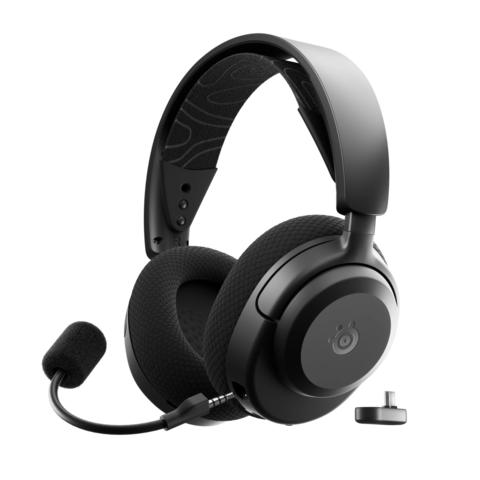
\includegraphics[width=\textwidth]{ressources/hs_2.png}
        \caption{Arctis Nova 3 Wireless}
    \end{subfigure}
    \hfill
    \begin{subfigure}[b]{0.25\textwidth}
        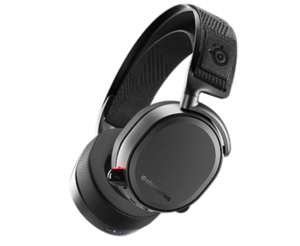
\includegraphics[width=\textwidth]{ressources/hs_3.png}
        \caption{Arctis Pro Wireless}
    \end{subfigure}
    \hfill
    \begin{subfigure}[b]{0.25\textwidth}
        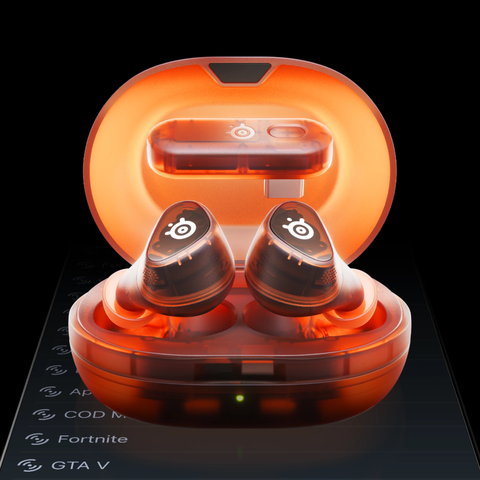
\includegraphics[width=\textwidth]{ressources/hs_1.png}
        \caption{Arctis GameBuds™ Glorange}
    \end{subfigure}
    \caption{SteelSeries Gaming Keyboards}
    \end{figure}
    \item \textbf{Mousepads:} Various sizes and materials optimized for different play styles.
    \item \textbf{Software:}
        \begin{itemize}
        \item \textbf{SteelSeries GG:} is an all-in-one software platform that brings together the various tools and services SteelSeries offers to enhance the gaming experience. It serves as the central hub for managing SteelSeries peripherals and includes multiple sub-applications.
        \item \textbf{SteelSeries Engine:} the part of GG that handles the core device configuration. It's used to customize settings for SteelSeries mice, keyboards, headsets, and other gear. Through Engine, users can adjust RGB lighting effects, set up macros, and fine-tune mouse sensitivity (DPI).
        \item SteelSeries' advanced audio suite built specifically for gamers who want precise control over their sound experience. It offers a powerful parametric equalizer that lets users independently customize audio for game sounds, voice chat, and microphone input.
        \item \textbf{SteelSeries Moments:} a gameplay capture tool within GG that automatically records key moments during gaming sessions. It can detect in-game events like kills, wins, or goals and save short clips around those events.
        \end{itemize} 
\end{itemize}

\subsection{Mission}
SteelSeries' mission is to create the best gaming gear in the world, empowering gamers to perform at their best, whether it is for professionals who seek perfection, or casuals who seek a sense of competition and completion. Its implication over the years in the esports scene has made it a trusted brand among professional gamers, and its commitment to innovation continues to drive the development of new products that enhance the gaming experience. Most notably, SKT Gaming, a professional esports organization, has been using SteelSeries products since 2012, and has won multiple championships in games like CS:GO and League of Legends etc.
\begin{figure}[h!]
    \centering
    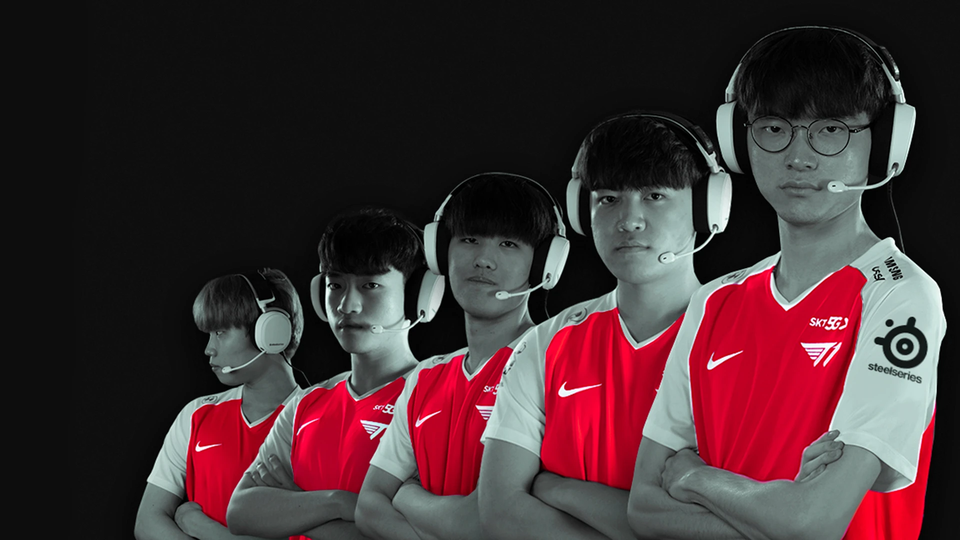
\includegraphics[width=0.7\textwidth]{ressources/sktt1.png}
    \caption{5x League of Legends World Champions SKT T1}
    \label{fig:5x League of Legends World Champions SKT T1}
\end{figure}
\section{Context \& Motivation}
\subsection{Feature Matching in Computer Vision}
\subsubsection{Definition}
Feature matching refers to the process of finding corresponding keypoints between two images of the same scene or object. These keypoints are distinctive image features, such as corners, edges, blobs, or regions with significant intensity changes that can be reliably identified in different images, even if those images have undergone transformations.
\subsection{How Feature Matching Works}
Feature matching typically involves several steps:
\begin{itemize}
    \item \textbf{Feature Extraction:} the initial step in feature matching, identifies distinctive, stable, and informative points of high-intensity variation—such as corners or edges—that are invariant to changes in rotation and scale.
    \item \textbf{Feature Description:} the process of computing a descriptor for each keypoint, which is a compact representation of the local image patch around the keypoint. This descriptor should be robust to changes in lighting, viewpoint, and other image transformations.
    \item \textbf{Feature Matching:} the final step involves finding correspondences between the keypoints in the two images based on their descriptors. This is typically done using techniques like nearest neighbor search, where the descriptor of each keypoint in one image is compared to all descriptors in the other image to find the best match.
\end{itemize}
\subsection{Scale Invariant Feature Transform}
In David G. Lowe’s 2004 paper, \textbf{SIFT} stands for \textit{Scale Invariant Feature Transform}, a method designed to detect and describe local features in images that remain stable across various transformations. The term encapsulates the core strengths of the algorithm:
\begin{itemize}
    \item \textbf{Scale Invariance:} SIFT demonstrates robustness against changes in image size by detecting extrema in scale-space using a Difference-of-Gaussian approach, making it effective across different zoom levels and image resolutions.
    
    \item \textbf{Transformation Resilience:} The algorithm maintains stability under various image transformations including rotation, scaling, partial changes in illumination, and viewpoint variations, ensuring reliable feature detection across different viewing conditions.
    
    \item \textbf{Distinctive Feature Representation:} SIFT identifies keypoints characterized by location, scale, orientation, and descriptor vectors based on local gradients, converting raw image data into a highly distinctive representation suitable for matching and recognition tasks.
\end{itemize}
Thus, SIFT provides a powerful framework for extracting and matching image features under challenging real-world conditions~\cite{lowe2004}.

\subsection{Challenges in Gaming Applications}
The primary challenge for image processing in real-time gaming is the extreme demand for \textbf{speed} and \textbf{low latency}, as any analysis must occur within a tight millisecond timeframe to avoid introducing lag. This becomes particularly difficult because image processing algorithms must \textit{compete for the same computational resources} that the game itself is using. This is not a minor issue, as modern AAA titles are specifically designed to \textbf{monopolize the GPU}. Games like \textit{Alan Wake 2} or \textit{Cyberpunk 2077}, with demanding features such as \textit{path tracing}, already push high-end graphics cards to their absolute limits merely to render the game world. Adding an additional workload like real-time image processing on top of this creates a severe \textbf{performance bottleneck}, forcing developers to make significant trade-offs between \textbf{accuracy} and \textbf{efficiency}, and to rely on \textit{incredibly lightweight algorithms} that won't cripple the game's frame rate.

\subsection{Limitations of Traditional Feature Matching Techniques}
Real-time applications, such as visual odometry (VO), SLAM, and gaming, require both high accuracy and extremely low latency; thus, feature matching algorithms must satisfy very stringent constraints. Traditional feature-based systems using SIFT or ORB work well for reliable and accurate matching under varying conditions, but they are slower because of the explicit data association steps involved. Such latency, however, is unacceptable when one has to make decisions within milliseconds. Zhao and Vela (2020) characterize this trade-off by stating, ``feature-based systems exhibit good performance, yet have higher latency due to explicit data association; direct \& semidirect systems have lower latency, but are inapplicable in some target scenarios or exhibit lower accuracy than feature-based ones''~\cite{zhao2020good}. This observation thus attests the traditional pipelines' readymade opposing factors-speed versus precision-while promoting lightweight or neural-assisted alternatives to ensure on-time delivery without siding with robustness.

\section{Project Objectives}
\subsection{Reproducing Feature Matching Techniques with Neural Networks}
Recent years have witnessed a surge of interest in leveraging neural networks to enhance image processing tasks, applications in this field range from image classification and object detection to semantic segmentation and vision language models. The idea is to use neural networks to learn the feature extraction and matching process, potentially leading to faster and more efficient algorithms. This project aims to explore the feasibility of using neural networks to reproduce traditional feature matching techniques, such as SIFT or ORB, while maintaining or improving their performance.
\subsection{Problem Statement}
This research investigates whether lightweight neural networks can effectively accelerate the most computationally intensive stages of traditional feature matching—specifically, keypoint detection and description, in SteelSeries Moments software. By integrating neural-assisted processing into a SIFT-based pipeline, the project aims to achieve substantial reductions in processing time without sacrificing matching accuracy or robustness. The findings will inform not only gaming software optimization but also the broader application of neural-accelerated methods in real-time computer vision, particularly on hardware-limited platforms.
\section{Industrial Relevance}
\subsection{Integration with SteelSeries Moments Software}
For a company like SteelSeries, which leads in the gaming and esports market, user experience is paramount. The primary goal of this project is to achieve a reduced processing time compared to the traditional SIFT method, currently in-use in the SteelSeries Moments software. This will allow users to quickly and efficiently analyze their gaming footage, enhancing their overall experience with the product without relying on heavy computational resources.
